

\chapter{The Memory System}
\label{sec:memory}

\section{The Cache Structure}

Each cache structure consists of the cache and multiple
queues. Figure~\ref{fig:cache} shows the overall cache structure in
the \SIM. There are two flows: 1) cache access flow: from a processor
or upper level cache miss, try to access the cache and 2) cache fill
flow: in case of a cache miss, the data is supplied from the lower
level cache or DRAM. Section~\ref{sec:queue} details all queues and
Section~\ref{sec:cache-flow} describes the flows between queues and a
cache.

\begin{figure*}[htb]
\centering
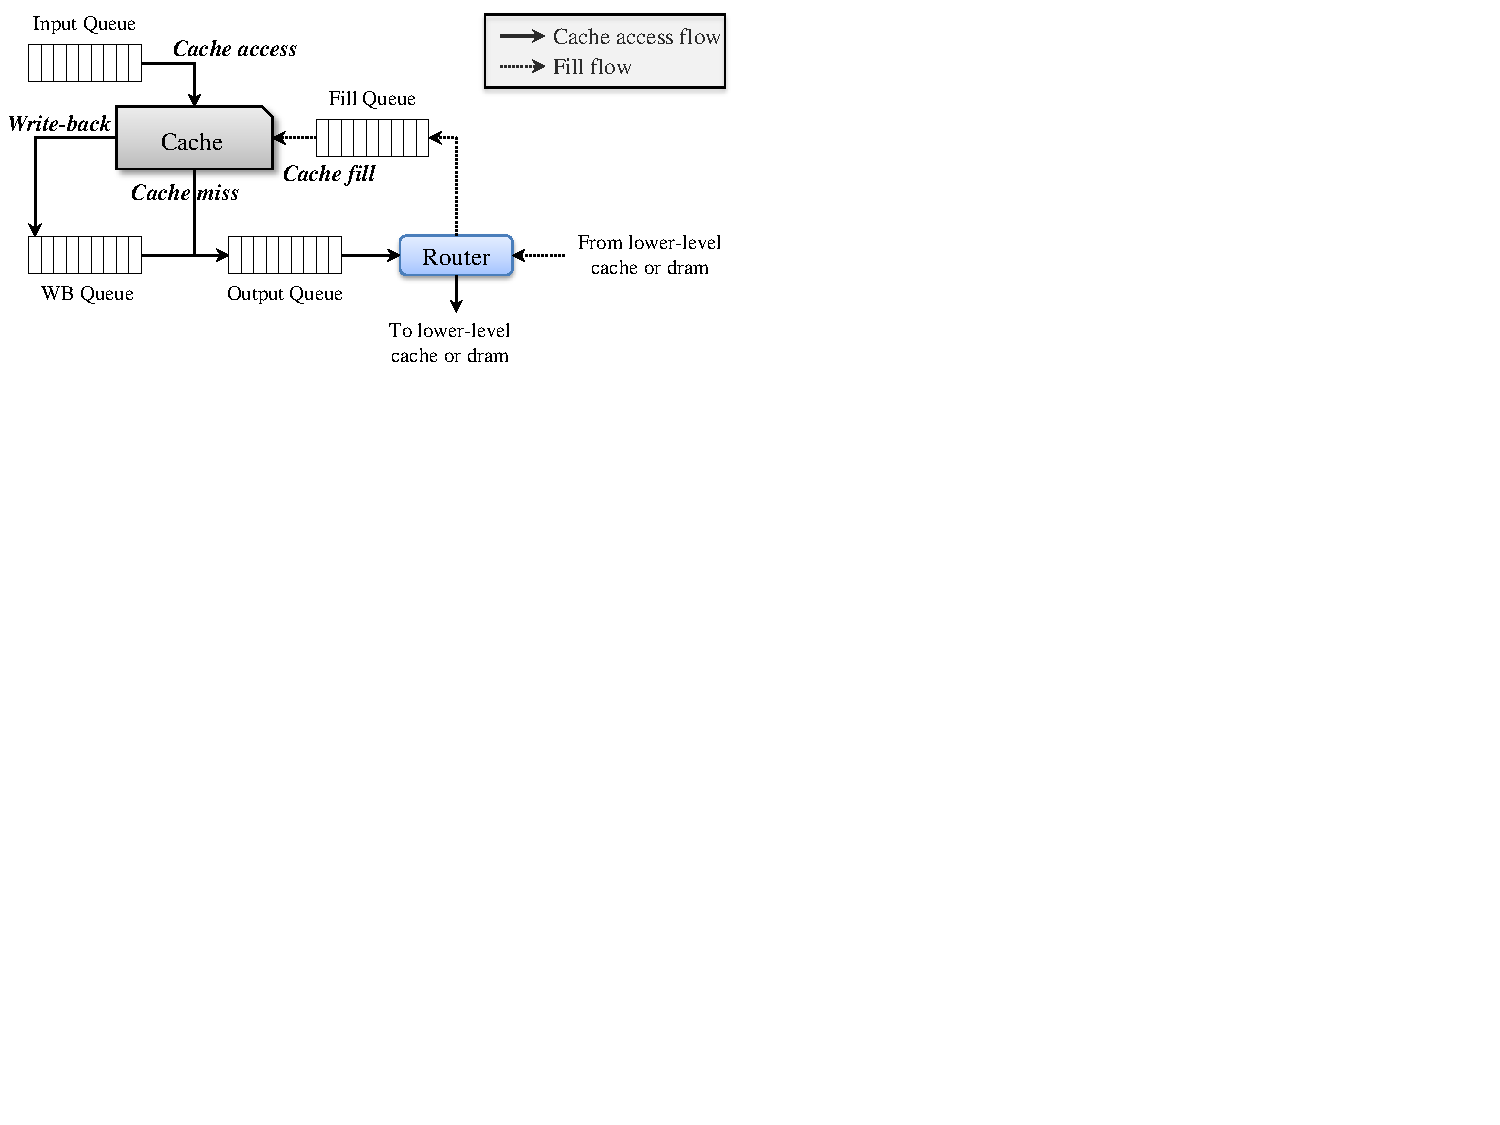
\includegraphics{figs/cache}
\caption{The cache structure.}
\label{fig:cache}
\end{figure*}


\subsection{The Queues}
\label{sec:queue}

All cache accesses flow from one queue to the other queue. 

\begin{itemize}
  \item input queue - to access a cache. Requests due to upper-level
  cache misses are inserted in this queue.

  \item output queue - as a result of a cache-miss, a request will be
  inserted into the output queue to be supplied data from the
  lower-level caches or DRAM.

  \item write-back queue - In \SIM, we model write-back caches. When a
  cache line is evicted and dirty, this line needs to be written back
  in the lower level. All write-back requests are initially inserted
  into the write-back queue.

  \item fill queue - requests in this queue tries to fill the data
  that is returned from the lower-level cache or DRAM.

  \item coherence queue - this queue is intended for handling
  coherence traffics, but this is currently not modeled.
\end{itemize}


\subsection{The Flows in the Cache Structure}
\label{sec:cache-flow}

\begin{itemize}

  \item Upper-level cache to input queue : upper-level cache miss

  \item input queue to cache : access the cache

  \item cache to output queue : cache miss and lower-level cache access

  \item cache to write-back queue : write-back requests

  \item write-back queue to output queue : to access lower-level cache

  \item output queue to the router : to access the lower-level cache
  through the on-chip interconnection network.

  \item router to the fill queue : the data from the lower-level cache
  or DRAM

\end{itemize}


\section{The Hierarchy}
\label{sec:memhierarchy}

\SIM maintains very flexible memory hierarchy. Each level of cache 
hierarchy is independent and \SIM defines the link between the
levels. Figure~\ref{fig:memory} shows the diagram of the memory
hierarchy in \SIM.

\begin{figure*}[htb]
\centering
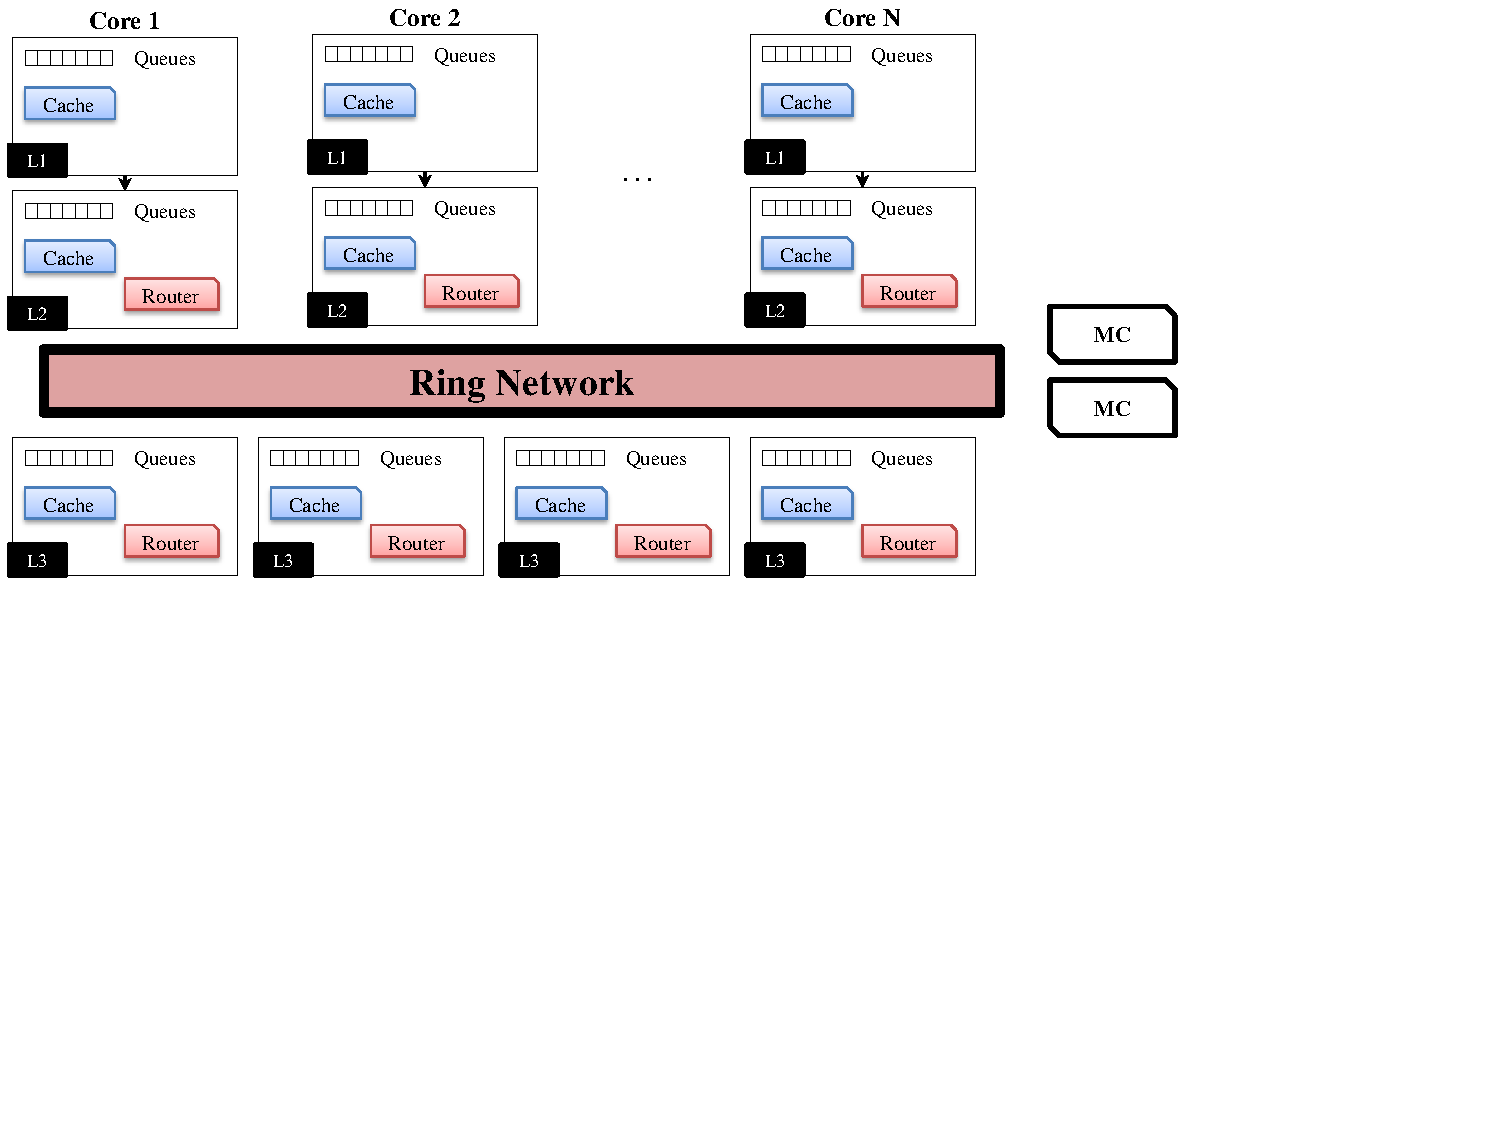
\includegraphics[width=6.5in]{figs/memory}
\caption{The memory system in \SIM.}
\label{fig:memory}
\end{figure*}



Here are some basics.


\begin{itemize}
  \item There are three levels (L1, L2, and L3) of caches in the \SIM
  although L2 cache might be disabled in some configurations.

  \item All these caches and memory controllers are connected via
  on-chip interconnection network (currently, the default topology is
  ring).

  \item L1 and L2 caches are always private to each processors.

  \item The local router within a cache structure is enabled when
  necessary.

  \item L3 cache is unified (shared by all cores), but tiled based on
  the static bank partition. In other words, address regions are
  statically partitioned and each tile is responsible for sub regions.

\end{itemize}


For example, Figure~\ref{fig:level2cache} shows the example of 2-level
caches. Even though there are 3-level caches, L2 cache is disabled and
only its router is used by the L1 cache to access the interconnection
network. Since there is no additional latency between L1 and L2, we
can flexibly configure 2-level caches.


\begin{figure*}[htb]
\centering
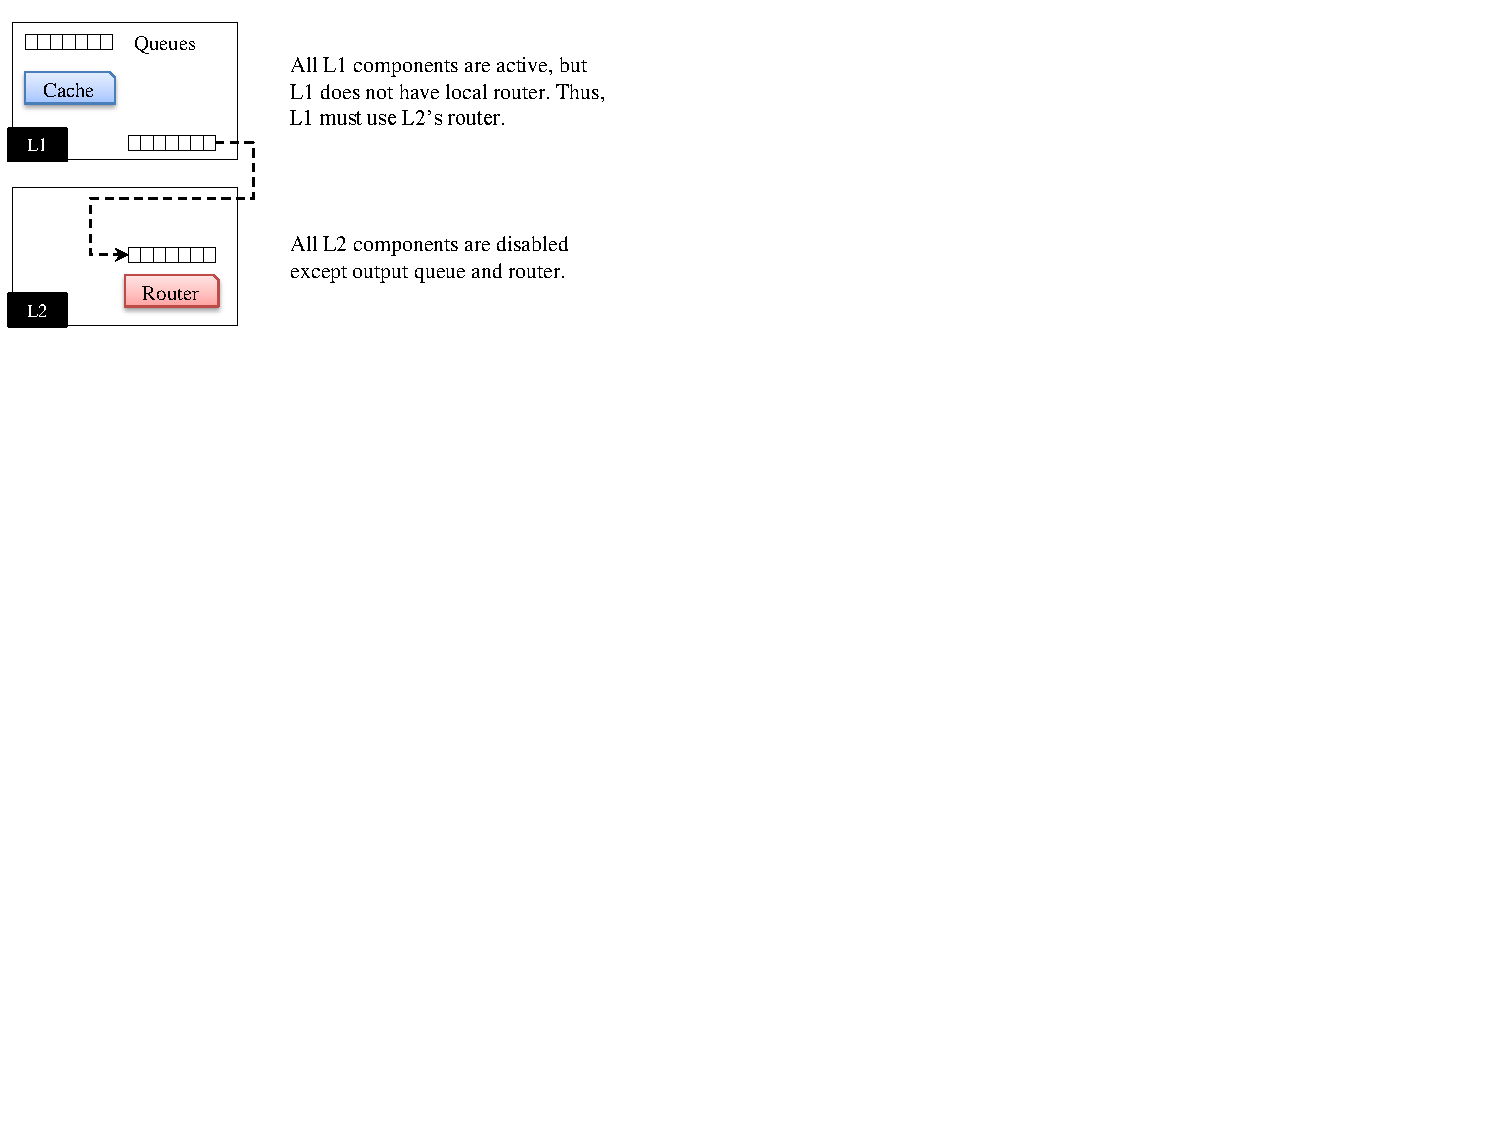
\includegraphics{figs/level2cache}
\caption{2-Level cache hierarchy.}
\label{fig:level2cache}
\end{figure*}


\section{How to Configure Cache Hierarchy} 

The cache hierarchy can be configured by setting 1) the link between
upper/lower level cache, 2) disability, and 3) router. The following
code is used in the \SIM cache initialization.

\begin{Verbatim}
void dcu_c::init(
  int next_id, // next level cache id
  int prev_id, // previous level cache id
  bool done, 
  bool coupled_up, // direct link with upper level cache
  bool coupled_down, // direct link with lower level cache
  bool disable, // disability
  bool has_router // router
);
\end{Verbatim}

\begin{description}
  \item[Router] When \textsf{has\_router} is set to \textit{false},
  the cache cannot directly access to the on-chip
  interconnection. Instead, it has to go through lower-level cache's
  interface. Therefore, \textsf{coupled\_down} must set
  to \textit{true} and appropriate \textsf{next\_id} must be set. In
  this way, the output queue of the cache is connected directly to the
  input queue of the next level (lower) cache.

  \item[Disability] When \textsf{disable} is set to \textit{true}, the
  cache is disabled. When a request is inserted from the upper level
  cache, it will be directly inserted into the output queue. This
  feature has been used for modeling 2-level cache hierarchy. As
  Figure~\ref{fig:level2cache} shown, L1 and L3 caches are active, but
  L2 cache is disabled. However, the L1 cache does not have a router,
  so it needs to use the router of the L2
  cache. Therefore, \textsf{has\_router} must be set to \textit{true}.

  \item[Link] As mentioned in the Section~\ref{sec:memhierarchy}, the
  L1 and L2 caches are always private to a processor. All L1 misses
  should go through the L2 cache without accessing the interconnection
  network. To this end, the direct link must be set between the L1 and
  L2 caches. Therefore, \textsf{coupled\_down} and \textsf{next\_id}
  must be set for the L1 cache and \textsf{coupled\_up}
  and \textsf{prev\_id} must be set for the L2 cache. Note that the
  link is always bi-directional.

\end{description}

\subsection{Example of Different Cache Hierarchy}

We provide several example of the cache hierarchy.

\begin{itemize}
\ignore{
  \item Intel Core~\cite{core2duo} microarchitecture has two-level of
  caches. The last-level cache might be tiled, but if the L2 cache
  tries to access the closest the L3 tile, it does not have to access
  through the interconnection. All communications will be made through
  the direct link. However, if the L2 cache accesses the remote L3
  tile, it goes through the interconnection. Note that the number of
  cores (L1 and L2 caches) and the number of the L3 tiles must be the
  same.

  \smallskip
  \begin{lstlisting}
  // class l2_coupled_local_c
  \end{lstlisting}
  \smallskip
}

  \item Intel Nehalem~\cite{nehalem} and Sandy
  Bridge~\cite{sandybridge} microarchitecture have three-level of
  caches. The last-level cache is tiled, but if the L2 cache tries to
  access the closest L3 tile, it does not have to access through the
  interconnection. All communications will be made through the direct
  link. However, if the L2 cache accesses the remote L3 tile, it goes
  through the interconnection. Note that the number of cores (L1 and
  L2 caches) and the number of the L3 tiles must be the same in this
  configuration.

\begin{Verbatim}
// class l3_coupled_network_c
for (int ii = 0; ii < m_num_core; ++ii) {
  // next_id, prev_id, done, coupled_up, coupled_down, disable, router
  m_l1_cache[ii]->init(ii, -1, false, false, TRUE, false, false);
  m_l2_cache[ii]->init(ii, ii, true,  TRUE,  TRUE, false, TRUE);
  m_l3_cache[ii]->init(-1, ii, false, TRUE,  false,false, TRUE);
}
\end{Verbatim}

  \item NVIDIA G80~\cite{g80} architecture does not have
  hardware-managed caches. Thus, all three levels are connected each
  other and disabled. Only the L3 cache has a router to access DRAM.

  \begin{Verbatim}
  // class no_cache_c
  for (int ii = 0; ii < m_num_core; ++ii) {
    // next_id, prev_id, done, coupled_up, coupled_down, disable, router
    m_l1_cache[ii]->init(ii, -1, false, false, TRUE,  TRUE, false);
    m_l2_cache[ii]->init(ii, ii, true,  TRUE,  TRUE,  TRUE, false);
    m_l3_cache[ii]->init(-1, ii, false, TRUE,  false, TRUE, TRUE);
  }
  \end{Verbatim}

  \item NVIDIA Fermi~\cite{fermi} architecture has private L1 cache
  and unified L2 cache shared by all cores. The L1 and L2 caches are
  linked. The L2 cache has been disabled, but has a router
  enabled. The L3 is not linked with others, but it is enabled and has
  a router.

  \begin{Verbatim}
  // class l2_decoupled_network_c
  // next_id, prev_id, done, coupled_up, coupled_down, disable, router
  for (int ii = 0; ii < m_num_core; ++ii) {
    m_l1_cache[ii]->init(ii, -1, false, false, TRUE,  false, false);
    m_l2_cache[ii]->init(-1, ii, true,  TRUE,  false, true,  true);
  }

  for (int ii = 0; ii < m_num_l3; ++ii) {
    // next_id, prev_id, done, coupled_up, coupled_down, disable, router
    m_l3_cache[ii]->init(-1, -1, false, false, false, false, true);
  }
  \end{Verbatim}
  
  \item In general 2-D Topology (Mesh, Torus), we assume each core has
  private L1 and L2 caches, but access to the L3 cache must be
  communicated through the interconnection network. The L1 and L2
  caches are both enabled and linked, but only the L2 cache has a
  router. The L3 cache is not linked with others and the communication
  is made through the interconnection network.

  \begin{Verbatim}
  // class l3_decoupled_network_c
  // next_id, prev_id, done, coupled_up, coupled_down, disable, router
  for (int ii = 0; ii < m_num_core; ++ii) {
    m_l1_cache[ii]->init(ii, -1, false, false, TRUE,  false, false);
    m_l2_cache[ii]->init(-1, ii, true,  TRUE,  false, false, TRUE);
  }

  for (int ii = 0; ii < m_num_l3; ++ii) {
    // next_id, prev_id, done, coupled_up, coupled_down, disable, router
    m_l3_cache[ii]->init(-1, -1, false, false, false, false, TRUE);
  }
  \end{Verbatim}
\end{itemize}

\section{DRAM Module} 

\SIM also models detail memory controllers: timing constraint, 
bandwidth, and scheduling. Section~\ref{sec:param-dram} describes how
to configure DRAM parameters.

The DRAM controller consists of multiple banks with one ore more
channels. Each bank has own request buffer and bank scheduler picked

\begin{itemize}
  \item The bank scheduler picks a request based on the policy (FCFS,
  FRFCFS, ...) if nothing is served now.

  \item The channel scheduler picks a request from command-ready banks
  (usually oldest request first). Based on the command, appropriate
  timing constraint is enforced to the bank.

  \item Once the column access signal is sent, the data is prepared
  from the DRAM chip (load) or the data is sent to the DRAM chip
  (store). Among multiple data-ready banks, the channel scheduler
  picks a request based on the policy (oldest-first).

  \item When the data is ready/sent for a request, the data is
  supplied to the cache (load) or the request is completed (store).

  \item If there are memory requests with the same address, these
  requests are merged into one dram request. 

\end{itemize}



% LocalWords:  prev bool microarchitecture Nehalem num init NVIDIA FCFS FRFCFS
